\documentclass[12pt,a4paper]{article}

\usepackage[utf8]{inputenc}
\usepackage[T1]{fontenc}
\usepackage[brazil]{babel}
\usepackage{geometry}
\usepackage{graphicx}
\usepackage{float}
\usepackage{array}
\usepackage{booktabs}
\usepackage[table]{xcolor}
\usepackage{longtable}
\usepackage{hyperref}
\usepackage{listings}
\usepackage{caption}
\usepackage{tikz}
\usepackage{microtype}
\usepackage{parskip}
\usepackage{enumitem}
\usepackage{fancyhdr}
\usepackage{titlesec}

\geometry{left=2.35cm,right=2.35cm,top=2.55cm,bottom=2.55cm}
\graphicspath{{img/}}

\hypersetup{
    colorlinks=true,
    linkcolor=blue!35!black,
    urlcolor=blue!45!black,
    citecolor=blue!35!black,
    pdftitle={Criação de Projeto no Quartus Prime para o Kit DE10-Lite},
    pdfauthor={Prof. Felipe Walter Dafico Pfrimer}
}
\urlstyle{same}

\definecolor{brand}{RGB}{28,74,118}
\definecolor{branddark}{RGB}{18,48,79}
\definecolor{accent}{RGB}{0,137,123}
\definecolor{softblue}{RGB}{233,241,249}
\definecolor{softgray}{RGB}{246,248,250}
\definecolor{codebg}{RGB}{247,249,252}
\definecolor{codeframe}{RGB}{190,205,222}
\definecolor{tablehead}{RGB}{28,74,118}
\definecolor{tablerow}{RGB}{239,245,250}
\definecolor{callout}{RGB}{190,35,35}

\setlength{\parindent}{0pt}
\setlength{\parskip}{0.62em}
\renewcommand{\arraystretch}{1.16}
\setlist[itemize]{topsep=0.35em,itemsep=0.22em,leftmargin=1.4cm}

\pagestyle{fancy}
\setlength{\headheight}{25pt}
\fancyhf{}
\lhead{\textsf{\small DE10-Lite e Quartus Prime}}
\rhead{\textsf{\small VHDL}}
\cfoot{\textsf{\small\thepage}}
\renewcommand{\headrulewidth}{0.4pt}
\renewcommand{\headrule}{\hbox to\headwidth{\color{brand}\leaders\hrule height \headrulewidth\hfill}}

\titleformat{\section}
  {\Large\sffamily\bfseries\color{branddark}}
  {\thesection}{0.8em}{}
  [\vspace{-0.25em}{\color{accent}\titlerule[0.8pt]}]
\titleformat{\subsection}
  {\large\sffamily\bfseries\color{brand}}
  {\thesubsection}{0.8em}{}
\titlespacing*{\section}{0pt}{1.4em}{0.75em}
\titlespacing*{\subsection}{0pt}{1.0em}{0.45em}

\renewcommand{\lstlistingname}{Código}
\renewcommand{\lstlistlistingname}{Lista de Códigos}
\captionsetup[table]{labelfont={bf,color=branddark},textfont=it,skip=6pt}
\captionsetup[figure]{labelfont={bf,color=branddark},textfont=it,skip=6pt}
\captionsetup[lstlisting]{labelfont={bf,color=branddark},textfont=it,skip=6pt}

\lstdefinestyle{quartuscode}{
    backgroundcolor=\color{codebg},
    frame=single,
    rulecolor=\color{codeframe},
    framerule=0.6pt,
    basicstyle=\ttfamily\small,
    keywordstyle=\color{brand}\bfseries,
    commentstyle=\color{green!35!black},
    stringstyle=\color{red!60!black},
    numbers=left,
    numberstyle=\tiny\color{gray},
    numbersep=8pt,
    stepnumber=1,
    breaklines=true,
    tabsize=4,
    showstringspaces=false,
    captionpos=b
}

\lstset{style=quartuscode}

\newcommand{\imagemquartus}[4]{
    \begin{figure}[H]
        \centering
        \includegraphics[width=#1\textwidth]{#2}
        \caption{#3}
        \label{#4}
    \end{figure}
}

\newcommand{\calloutstyle}{
    \tikzset{
        calloutbox/.style={
            draw=callout,
            fill=white,
            rounded corners=3pt,
            line width=0.8pt,
            font=\small\sffamily\bfseries,
            align=center,
            inner sep=3.5pt
        },
        calloutarrow/.style={
            ->,
            >=stealth,
            draw=callout,
            line width=1.2pt
        }
    }
}

\newcommand{\caixaatencao}[1]{
    \begin{center}
    \setlength{\fboxsep}{8pt}
    \fcolorbox{callout}{softgray}{
        \begin{minipage}{0.90\textwidth}
        \raggedright
        \textbf{\textsf{Atenção}}\\[0.35em]
        #1
        \end{minipage}
    }
    \end{center}
}

\newcommand{\caixaresumo}[2]{
    \begin{center}
    \setlength{\fboxsep}{8pt}
    \fcolorbox{accent}{softblue}{
        \begin{minipage}{0.90\textwidth}
        \raggedright
        \textbf{\textsf{#1}}\\[0.35em]
        #2
        \end{minipage}
    }
    \end{center}
}

\title{\textbf{Criação de Projeto no Quartus Prime para o Kit DE10-Lite}\\
\large Top-level design em VHDL com pinos configurados}
\author{Prof. Felipe Walter Dafico Pfrimer}
\date{\today}

\begin{document}
\pagenumbering{gobble}

\begin{titlepage}
\thispagestyle{empty}
\begin{tikzpicture}[remember picture,overlay]
    \fill[branddark] (current page.north west) rectangle (current page.south east);
    \fill[accent] (current page.north west) rectangle ([yshift=-0.22cm]current page.north east);
    \fill[accent] ([yshift=0.22cm]current page.south west) rectangle (current page.south east);
    \draw[white, line width=0.7pt, opacity=0.45]
        ([xshift=1.35cm,yshift=-1.35cm]current page.north west)
        rectangle
        ([xshift=-1.35cm,yshift=1.35cm]current page.south east);
\end{tikzpicture}

\vspace*{2.2cm}
{\sffamily\color{white}
{\Large Apostila prática}\\[1.2cm]
{\Huge\bfseries Criação de Projeto}\\[0.18cm]
{\Huge\bfseries no Quartus Prime}\\[0.45cm]
{\LARGE para o Kit DE10-Lite}\\[1.0cm]
{\Large Top-level design em VHDL com pinos configurados}\\[2.0cm]
{\large Prof. Felipe Walter Dafico Pfrimer}
}

\vfill

\colorbox{white}{
    \parbox{0.88\textwidth}{
        \color{branddark}
        \textbf{\textsf{Objetivo}}\\[0.35em]
        Esta apostila apresenta um fluxo prático para criar um projeto no Quartus Prime Lite para o kit DE10-Lite, selecionar corretamente a placa e o dispositivo FPGA, criar um top-level design em VHDL e configurar os pinos físicos. O exemplo principal implementa um contador decimal de 00 a 99, com reset, carga paralela pelas chaves e exibição nos displays de sete segmentos.
    }
}

\vspace*{1.0cm}
{\sffamily\color{white}\today}
\end{titlepage}

\pagenumbering{roman}
\tableofcontents
\newpage
\pagenumbering{arabic}

\section{Materiais necessários}

Para acompanhar o roteiro, utilize:

\begin{itemize}
    \item Kit FPGA Terasic DE10-Lite.
    \item Cabo USB conectado à porta USB-Blaster da placa.
    \item Quartus Prime Lite instalado.
    \item Arquivo VHDL do top-level design.
    \item Tabela de pinos da DE10-Lite ou arquivo \texttt{.qsf} com os pinos já atribuídos.
\end{itemize}

\caixaresumo{Checklist rápido antes de começar}{
\begin{itemize}
    \item A placa está conectada pela porta USB-Blaster.
    \item O Quartus Prime Lite abre sem solicitar instalação adicional do dispositivo MAX 10.
    \item A pasta do projeto foi criada em um caminho simples, sem acentos e sem espaços.
    \item O nome escolhido para a entidade principal será repetido exatamente no arquivo VHDL.
\end{itemize}
}

\section{Informações do kit DE10-Lite}

O kit DE10-Lite utiliza um FPGA da família MAX 10. Para o projeto apresentado nesta apostila, a seleção do dispositivo deve seguir a Tabela~\ref{tab:dispositivo}.

\begin{table}[H]
\centering
\caption{Configurações principais do projeto para a DE10-Lite.}
\label{tab:dispositivo}
\rowcolors{2}{tablerow}{white}
\begin{tabular}{>{\bfseries}p{0.35\textwidth}p{0.5\textwidth}}
\toprule
\rowcolor{tablehead}
\color{white}\textbf{Item} & \color{white}\textbf{Configuração} \\
\midrule
Família & MAX 10 \\
Dispositivo & \texttt{10M50DAF484C6GES} \\
Placa & MAX 10 DE10-Lite \\
Entidade de topo do exemplo & \texttt{Contador\_DE10\_Lite} \\
Linguagem usada na apostila & VHDL \\
\bottomrule
\end{tabular}
\end{table}

O nome da entidade de topo em VHDL precisa coincidir com o nome definido no Quartus em \textit{Top-Level Entity}. Neste exemplo, será usado \texttt{Contador\_DE10\_Lite}. Se houver diferença de maiúsculas, minúsculas ou sublinhados, o Quartus poderá não encontrar a entidade principal durante a compilação.

\caixaatencao{O Quartus diferencia letras maiúsculas, minúsculas e sublinhados no nome da entidade. Se o projeto estiver configurado como \texttt{Contador\_DE10\_Lite}, a declaração VHDL deve usar exatamente esse nome.}

\section{Criação do projeto no Quartus}

Ao abrir o Quartus Prime Lite, a tela inicial apresenta o botão \textit{New Project Wizard}, indicado na Figura~\ref{fig:tela-inicial}. Clique nele para iniciar a criação do projeto.

\begin{figure}[H]
\centering
\calloutstyle
\begin{tikzpicture}
    \node[anchor=south west,inner sep=0] (img) at (0,0)
        {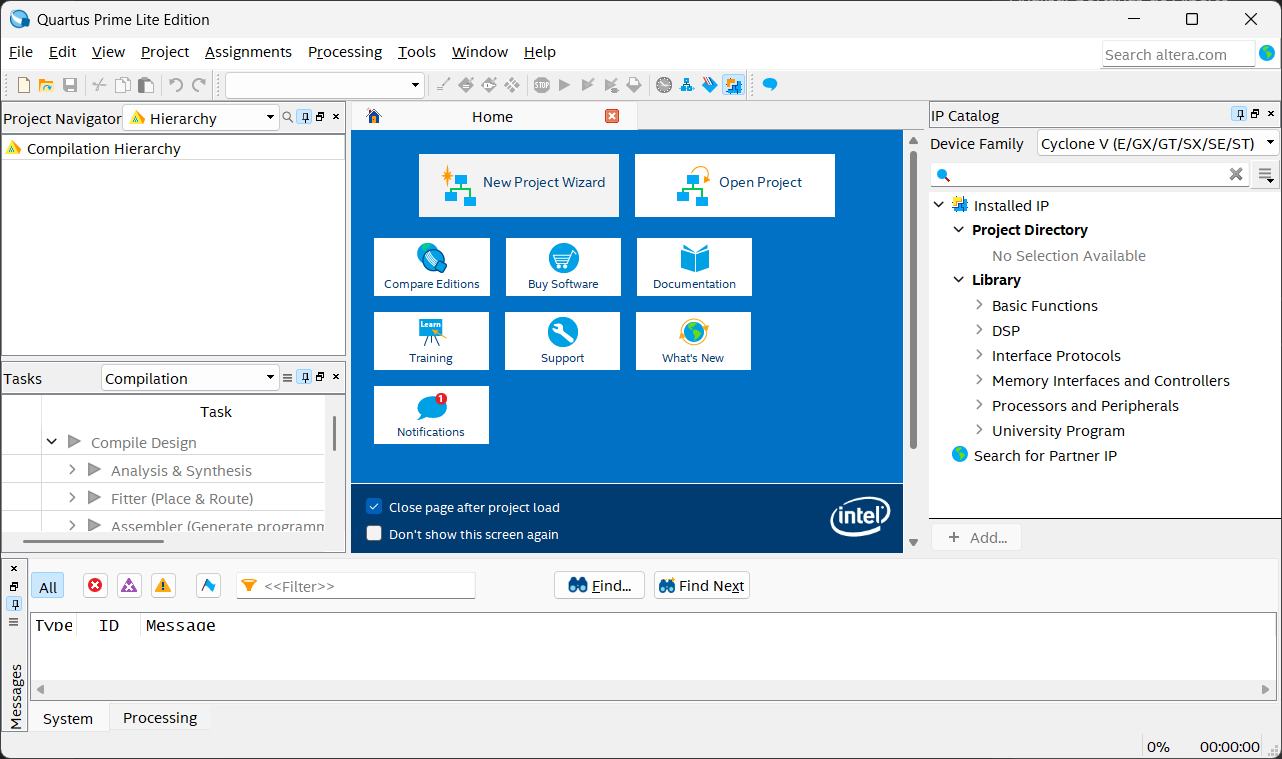
\includegraphics[width=0.95\textwidth]{image1.png}};
    \begin{scope}[x={(img.south east)},y={(img.north west)}]
        \node[calloutbox] (wiz) at (0.63,0.77) {Novo\\projeto};
        \draw[calloutarrow] (wiz.west) -- (0.41,0.76);
    \end{scope}
\end{tikzpicture}
\caption{Tela inicial do Quartus Prime Lite.}
\label{fig:tela-inicial}
\end{figure}

A primeira janela do assistente é uma introdução ao fluxo de criação, como mostra a Figura~\ref{fig:introducao-assistente}. Clique em \textit{Next} para avançar.

\imagemquartus{0.75}{image2.png}{Introdução do assistente \textit{New Project Wizard}.}{fig:introducao-assistente}

Na etapa da Figura~\ref{fig:nome-projeto}, escolha a pasta do projeto e informe o nome da entidade principal. O Código~\ref{cod:organizacao} mostra uma sugestão de preenchimento.

\begin{figure}[H]
\centering
\calloutstyle
\begin{tikzpicture}
    \node[anchor=south west,inner sep=0] (img) at (0,0)
        {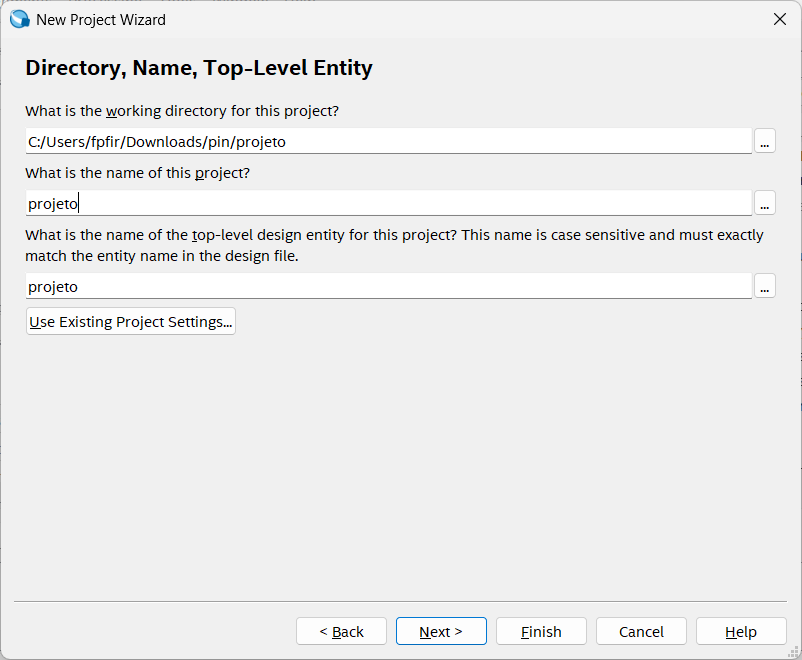
\includegraphics[width=0.75\textwidth]{image3.png}};
    \begin{scope}[x={(img.south east)},y={(img.north west)}]
        \node[calloutbox] (top) at (0.74,0.50) {Nome da\\entidade};
        \draw[calloutarrow] (top.west) -- (0.18,0.57);
    \end{scope}
\end{tikzpicture}
\caption{Definição do diretório, nome do projeto e entidade de topo.}
\label{fig:nome-projeto}
\end{figure}

\begin{lstlisting}[caption={Exemplo de organização inicial do projeto.},label={cod:organizacao}]
Pasta do projeto: C:\Projetos\DE10_Lite
Nome do projeto: projeto
Top-level entity: Contador_DE10_Lite
\end{lstlisting}

Na etapa de tipo de projeto, selecione \textit{Empty project}, conforme a Figura~\ref{fig:tipo-projeto}. Essa opção cria um projeto vazio, no qual o arquivo VHDL será adicionado manualmente.

\imagemquartus{0.75}{image4.png}{Seleção do tipo de projeto.}{fig:tipo-projeto}

Caso já exista um arquivo VHDL pronto, adicione-o na tela da Figura~\ref{fig:inclusao-arquivos}. Se ainda não existir, avance sem adicionar arquivos e crie o VHDL depois.

\imagemquartus{0.75}{image5.png}{Inclusão de arquivos existentes no projeto.}{fig:inclusao-arquivos}

Na etapa de dispositivo, a tela pode aparecer inicialmente com outra família selecionada, como na Figura~\ref{fig:selecao-dispositivo}. Selecione a família \texttt{MAX 10} para trabalhar com a DE10-Lite.

\imagemquartus{0.90}{image6.png}{Tela de seleção de família, dispositivo e placa.}{fig:selecao-dispositivo}

Na aba \textit{Board}, selecione a placa \textit{MAX 10 DE10-Lite}, como indicado na Figura~\ref{fig:selecao-placa}. Essa tela também possui a opção \textit{Create top-level design file}.

\begin{figure}[H]
\centering
\calloutstyle
\begin{tikzpicture}
    \node[anchor=south west,inner sep=0] (img) at (0,0)
        {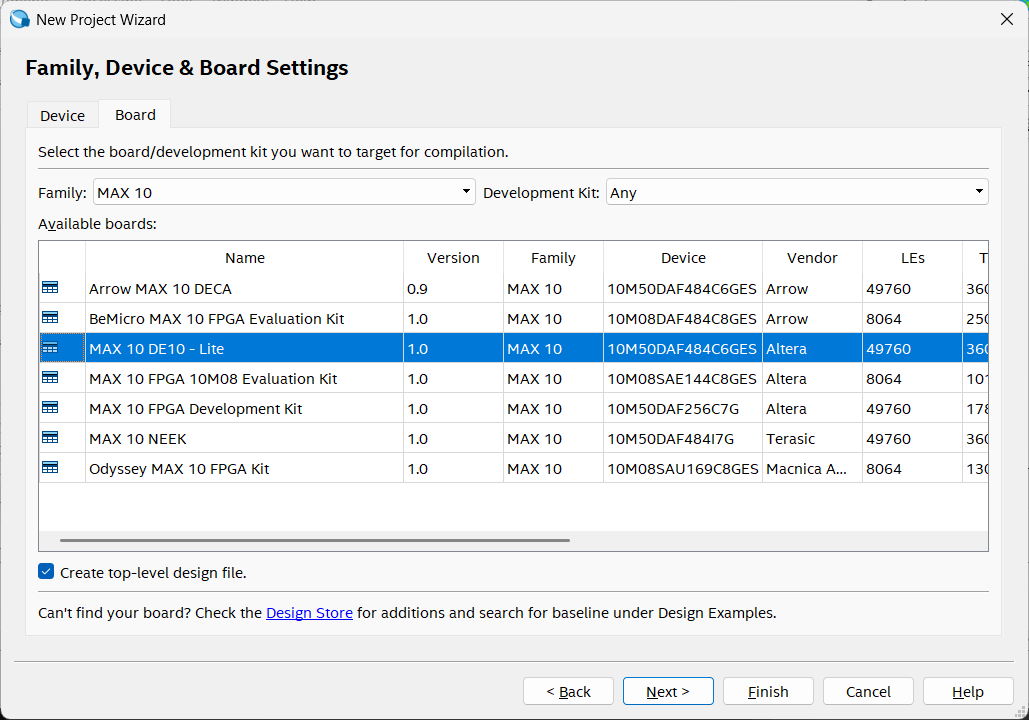
\includegraphics[width=0.90\textwidth]{image7.png}};
    \begin{scope}[x={(img.south east)},y={(img.north west)}]
        \node[calloutbox] (board) at (0.82,0.64) {Placa\\DE10-Lite};
        \draw[calloutarrow] (board.west) -- (0.23,0.52);
        \node[calloutbox] (auto) at (0.49,0.08) {Arquivo padrão\\Golden Top};
        \draw[calloutarrow] (auto.west) -- (0.05,0.21);
    \end{scope}
\end{tikzpicture}
\caption{Seleção da placa e opção de criação automática do arquivo de topo.}
\label{fig:selecao-placa}
\end{figure}

Quando a opção \textit{Create top-level design file} da Figura~\ref{fig:selecao-placa} fica marcada, o Quartus/Terasic pode criar automaticamente o arquivo \texttt{DE10\_LITE\_Golden\_Top.v}. Nesta apostila, esse arquivo não será usado como descrição do circuito. Ele servirá apenas como referência para consultar nomes de portas da placa, como \texttt{SW}, \texttt{KEY}, \texttt{LEDR}, \texttt{HEX0}, \texttt{HEX1} e \texttt{MAX10\_CLK1\_50}. O circuito do aluno será escrito em VHDL, em um arquivo separado.

Um detalhe importante: se o top-level em VHDL usar exatamente os mesmos nomes de portas que aparecem no Golden Top e que já estão atribuídos no projeto, o Quartus consegue aproveitar as configurações de pinos já existentes. Nesse caso, não é necessário refazer manualmente essas atribuições no Pin Planner nem reescrevê-las no arquivo \texttt{.qsf}. A configuração manual só será necessária quando o projeto não tiver essas atribuições prontas ou quando os nomes das portas forem diferentes.

\caixaresumo{Papel do Golden Top}{
O arquivo \texttt{DE10\_LITE\_Golden\_Top.v} pode ser útil como uma lista de nomes oficiais das portas da placa. Nesta apostila, ele não descreve o circuito e não precisa ser chamado pelo VHDL. O top-level real será o arquivo \texttt{Contador\_DE10\_Lite.vhd}.
}

\section{Criação do arquivo VHDL}

Com o projeto aberto, crie um novo arquivo em:

\begin{center}
\texttt{File > New > VHDL File}
\end{center}

A Figura~\ref{fig:novo-vhdl} mostra a janela de criação de arquivos do Quartus. Nela, selecione \textit{VHDL File} dentro do grupo \textit{Design Files} e clique em \textit{OK}.

\begin{figure}[H]
\centering
\calloutstyle
\begin{tikzpicture}
    \node[anchor=south west,inner sep=0] (img) at (0,0)
        {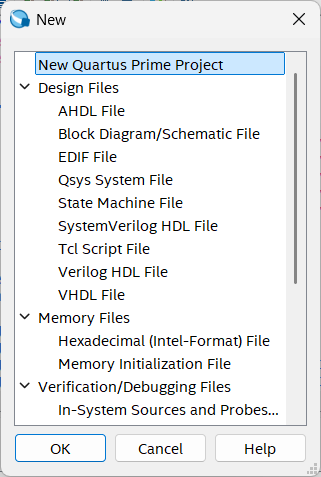
\includegraphics[width=0.42\textwidth]{image19.png}};
    \begin{scope}[x={(img.south east)},y={(img.north west)}]
        \node[calloutbox] (vhdl) at (0.76,0.42) {Arquivo\\VHDL};
        \draw[calloutarrow] (vhdl.west) -- (0.30,0.37);
        \node[calloutbox] (ok) at (0.36,0.10) {Confirmar};
        \draw[calloutarrow] (ok.south) -- (0.19,0.055);
    \end{scope}
\end{tikzpicture}
\caption{Seleção da opção \textit{VHDL File} para criar o arquivo do contador.}
\label{fig:novo-vhdl}
\end{figure}

Após criar o arquivo da Figura~\ref{fig:novo-vhdl}, salve-o como:

\begin{center}
\texttt{Contador\_DE10\_Lite.vhd}
\end{center}

Depois de salvar o arquivo, adicione-o ao projeto se necessário. A Figura~\ref{fig:projeto-aberto} mostra um projeto aberto após a criação automática do Golden Top. Note que o arquivo \texttt{DE10\_LITE\_Golden\_Top.v} aparece na lista, mas ele será usado apenas para consulta.

\imagemquartus{0.95}{image8.png}{Projeto aberto com o arquivo Golden Top criado automaticamente.}{fig:projeto-aberto}

A Figura~\ref{fig:golden-top} mostra o Golden Top aberto no editor. O trecho exibido é útil porque mostra nomes de portas da placa, por exemplo \texttt{HEX0}, \texttt{HEX1}, \texttt{KEY}, \texttt{LEDR} e \texttt{SW}. No VHDL do contador, não é necessário copiar todas essas portas; basta declarar as portas realmente usadas.

\begin{figure}[H]
\centering
\calloutstyle
\begin{tikzpicture}
    \node[anchor=south west,inner sep=0] (img) at (0,0)
        {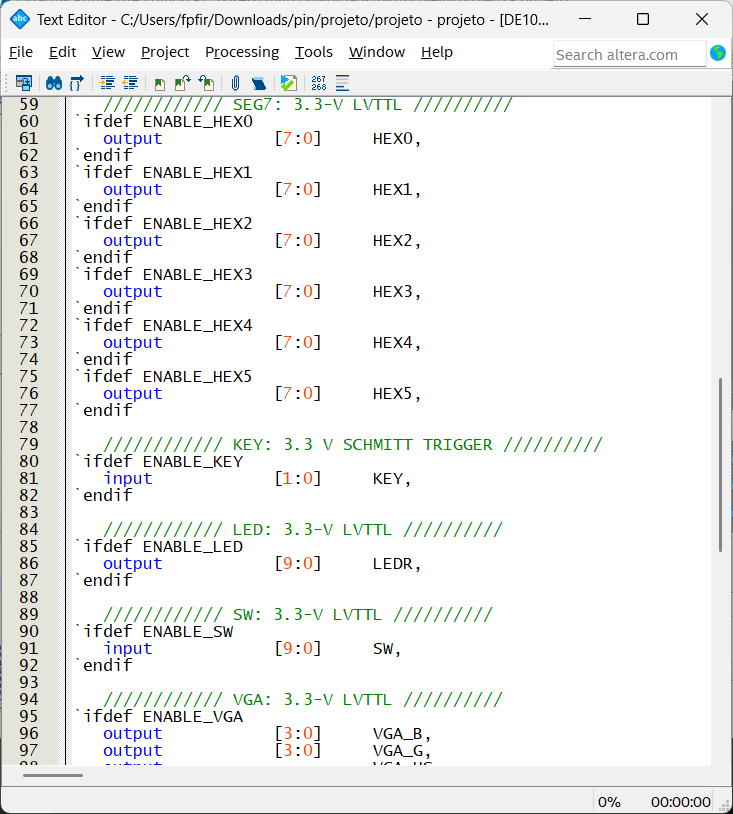
\includegraphics[width=0.72\textwidth]{image9.png}};
    \begin{scope}[x={(img.south east)},y={(img.north west)}]
        \node[calloutbox] (ports) at (0.78,0.27) {Nomes dos\\ports};
        \draw[calloutarrow] (ports.west) -- (0.50,0.59);
        \draw[calloutarrow] (ports.west) -- (0.50,0.73);
    \end{scope}
\end{tikzpicture}
\caption{Arquivo Golden Top usado apenas como referência para os nomes das portas.}
\label{fig:golden-top}
\end{figure}

\section{Top-level design em VHDL}

O top-level design é a entidade principal do projeto. Ele declara quais sinais entram e saem do FPGA e permite que o Quartus relacione esses sinais aos pinos físicos da placa. Neste exemplo, serão usados os sinais da Tabela~\ref{tab:sinais}.

\begin{table}[H]
\centering
\caption{Sinais usados pelo contador em VHDL.}
\label{tab:sinais}
\rowcolors{2}{tablerow}{white}
\begin{tabular}{>{\ttfamily}p{0.22\textwidth}p{0.22\textwidth}p{0.42\textwidth}}
\toprule
\rowcolor{tablehead}
\color{white}\textbf{Sinal} & \color{white}\textbf{Direção} & \color{white}\textbf{Função no circuito} \\
\midrule
MAX10\_CLK1\_50 & Entrada & Clock de 50 MHz da placa. \\
KEY(0) & Entrada & Reset ativo em nível baixo. \\
KEY(1) & Entrada & Carga paralela ativa em nível baixo. \\
SW(7 downto 0) & Entrada & Valor BCD para carga paralela: dezenas em \texttt{SW(7 downto 4)} e unidades em \texttt{SW(3 downto 0)}. \\
HEX0 & Saída & Display de sete segmentos das unidades. \\
HEX1 & Saída & Display de sete segmentos das dezenas. \\
LEDR & Saída & LEDs usados para visualizar as chaves. \\
\bottomrule
\end{tabular}
\end{table}

Os botões \texttt{KEY} e os displays \texttt{HEX} da DE10-Lite são ativos em nível baixo. Isso significa que o botão pressionado gera valor lógico \texttt{'0'}, e um segmento do display acende quando recebe \texttt{'0'}.

O Código~\ref{cod:vhdl-contador} implementa um contador decimal de 00 a 99. O contador avança aproximadamente uma vez por segundo, usando o clock de 50 MHz da placa. O botão \texttt{KEY(0)} zera a contagem, enquanto \texttt{KEY(1)} carrega o valor informado pelas chaves \texttt{SW(7 downto 0)}.

\begin{lstlisting}[language=VHDL,caption={Top-level design em VHDL: contador decimal com reset e carga paralela.},label={cod:vhdl-contador}]
library ieee;
use ieee.std_logic_1164.all;
use ieee.numeric_std.all;

entity Contador_DE10_Lite is
    port (
        MAX10_CLK1_50 : in  std_logic;
        KEY           : in  std_logic_vector(1 downto 0);
        SW            : in  std_logic_vector(9 downto 0);
        LEDR          : out std_logic_vector(9 downto 0);
        HEX0          : out std_logic_vector(7 downto 0);
        HEX1          : out std_logic_vector(7 downto 0)
    );
end entity Contador_DE10_Lite;

architecture rtl of Contador_DE10_Lite is
    constant DIVISOR_1HZ : natural := 50000000;

    signal div_count : natural range 0 to DIVISOR_1HZ - 1 := 0;
    signal tick_1hz  : std_logic := '0';
    signal unidade   : unsigned(3 downto 0) := (others => '0');
    signal dezena    : unsigned(3 downto 0) := (others => '0');

    function seg7(bcd : unsigned(3 downto 0)) return std_logic_vector is
    begin
        case bcd is
            when "0000" => return "11000000"; -- 0
            when "0001" => return "11111001"; -- 1
            when "0010" => return "10100100"; -- 2
            when "0011" => return "10110000"; -- 3
            when "0100" => return "10011001"; -- 4
            when "0101" => return "10010010"; -- 5
            when "0110" => return "10000010"; -- 6
            when "0111" => return "11111000"; -- 7
            when "1000" => return "10000000"; -- 8
            when "1001" => return "10010000"; -- 9
            when others => return "11111111"; -- apagado
        end case;
    end function;
begin
    LEDR <= SW;

    process (MAX10_CLK1_50)
    begin
        if rising_edge(MAX10_CLK1_50) then
            if div_count = DIVISOR_1HZ - 1 then
                div_count <= 0;
                tick_1hz  <= '1';
            else
                div_count <= div_count + 1;
                tick_1hz  <= '0';
            end if;
        end if;
    end process;

    process (MAX10_CLK1_50)
        variable carga_unidade : unsigned(3 downto 0);
        variable carga_dezena  : unsigned(3 downto 0);
    begin
        if rising_edge(MAX10_CLK1_50) then
            carga_unidade := unsigned(SW(3 downto 0));
            carga_dezena  := unsigned(SW(7 downto 4));

            if KEY(0) = '0' then
                unidade <= (others => '0');
                dezena  <= (others => '0');
            elsif KEY(1) = '0' then
                if carga_unidade <= to_unsigned(9, 4) and
                   carga_dezena <= to_unsigned(9, 4) then
                    unidade <= carga_unidade;
                    dezena  <= carga_dezena;
                else
                    unidade <= (others => '0');
                    dezena  <= (others => '0');
                end if;
            elsif tick_1hz = '1' then
                if unidade = to_unsigned(9, 4) then
                    unidade <= (others => '0');

                    if dezena = to_unsigned(9, 4) then
                        dezena <= (others => '0');
                    else
                        dezena <= dezena + 1;
                    end if;
                else
                    unidade <= unidade + 1;
                end if;
            end if;
        end if;
    end process;

    HEX0 <= seg7(unidade);
    HEX1 <= seg7(dezena);
end architecture rtl;
\end{lstlisting}

\section{Definição da entidade principal}

Depois de salvar o arquivo VHDL, confirme se ele está definido como top-level:

\begin{center}
\texttt{Project > Set as Top-Level Entity}
\end{center}

Uma forma prática de fazer isso é clicar com o botão direito sobre o arquivo VHDL e escolher \textit{Set as Top-Level Entity}, como mostra a Figura~\ref{fig:set-top-level}. Também é possível verificar essa configuração em:

\begin{figure}[H]
\centering
\calloutstyle
\begin{tikzpicture}
    \node[anchor=south west,inner sep=0] (img) at (0,0)
        {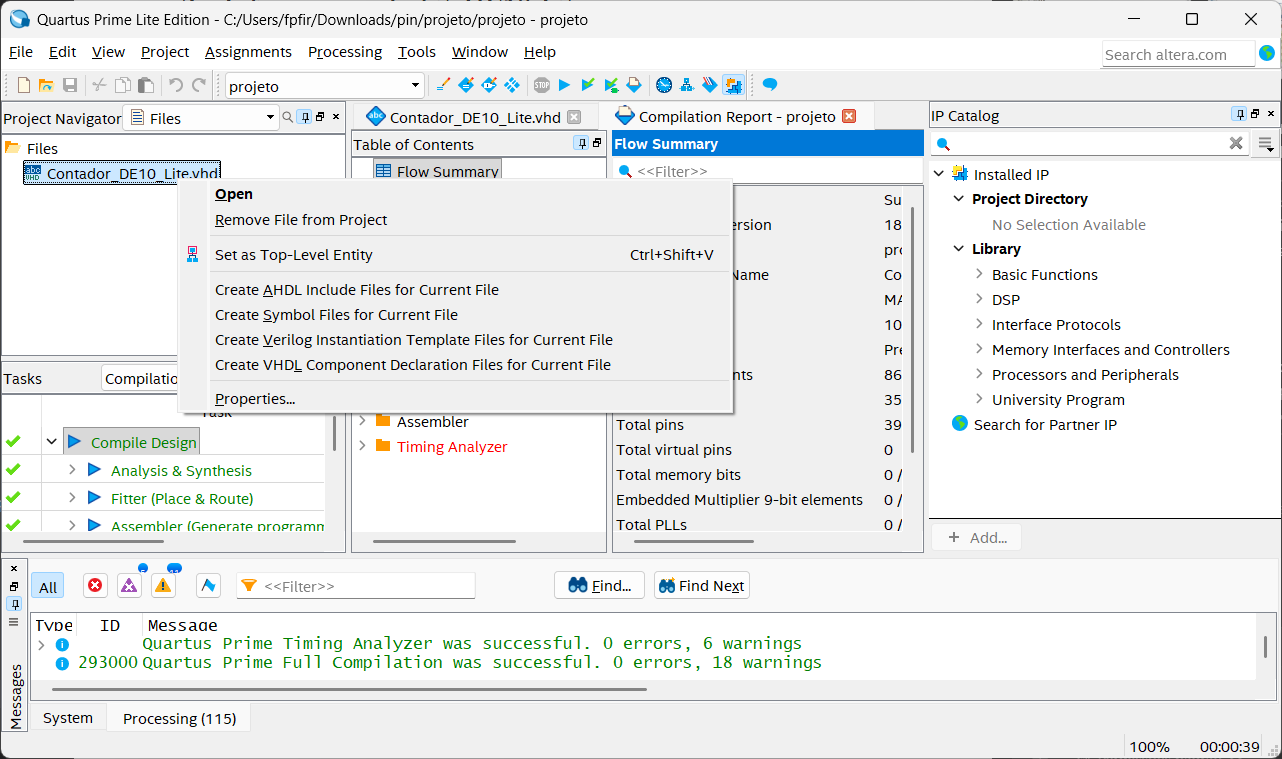
\includegraphics[width=0.95\textwidth]{image13.png}};
    \begin{scope}[x={(img.south east)},y={(img.north west)}]
        \node[calloutbox] (menu) at (0.43,0.68) {Definir como\\top-level};
        \draw[calloutarrow] (menu.south) -- (0.32,0.665);
        \node[calloutbox] (file) at (0.20,0.84) {Arquivo\\VHDL};
        \draw[calloutarrow] (file.south) -- (0.095,0.77);
    \end{scope}
\end{tikzpicture}
\caption{Definição do arquivo VHDL como entidade principal do projeto.}
\label{fig:set-top-level}
\end{figure}

Além do menu de contexto da Figura~\ref{fig:set-top-level}, também é possível verificar essa configuração em:

\begin{center}
\texttt{Assignments > Settings > General > Top-level entity}
\end{center}

O nome configurado deve ser o mesmo da entidade do Código~\ref{cod:vhdl-contador}: \texttt{Contador\_DE10\_Lite}.

\section{Configuração dos pinos}

A configuração dos pinos pode ser feita pela interface gráfica, usando o \textit{Pin Planner}, ou diretamente pelo arquivo \texttt{.qsf}. A Figura~\ref{fig:pin-planner} mostra o Pin Planner com atribuições de displays de sete segmentos.

\begin{figure}[H]
\centering
\calloutstyle
\begin{tikzpicture}
    \node[anchor=south west,inner sep=0] (img) at (0,0)
        {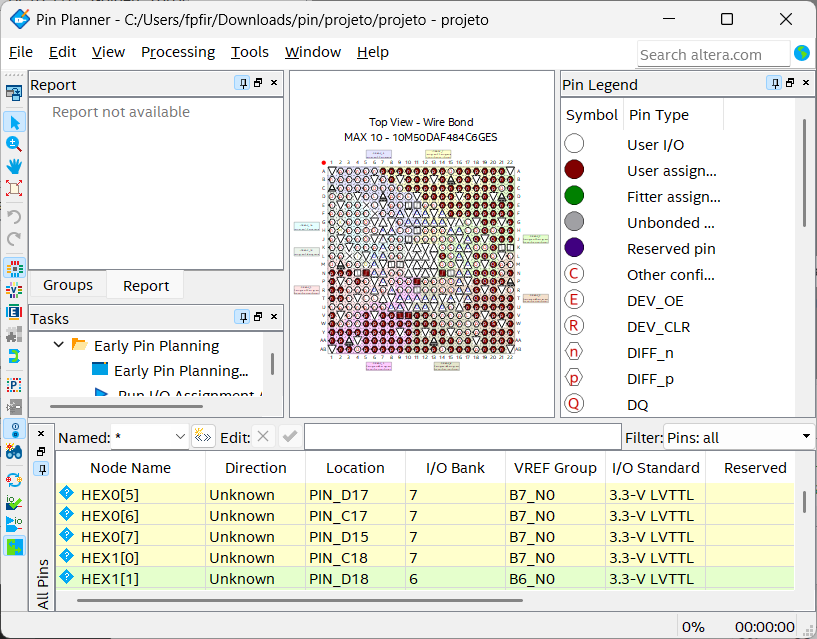
\includegraphics[width=0.78\textwidth]{image10.png}};
    \begin{scope}[x={(img.south east)},y={(img.north west)}]
        \node[calloutbox] (table) at (0.20,0.70) {Tabela de\\pinos};
        \draw[calloutarrow] (table.south) -- (0.35,0.22);
        \node[calloutbox] (std) at (0.84,0.70) {Padrão\\elétrico};
        \draw[calloutarrow] (std.south) -- (0.77,0.22);
    \end{scope}
\end{tikzpicture}
\caption{Pin Planner usado para associar sinais aos pinos físicos.}
\label{fig:pin-planner}
\end{figure}

No Pin Planner, cada sinal do top-level deve receber uma localização física, como \texttt{PIN\_A8}, e um padrão elétrico de entrada e saída, como \texttt{3.3-V LVTTL}. Para os botões \texttt{KEY}, utiliza-se \texttt{3.3 V SCHMITT TRIGGER}. A Tabela~\ref{tab:pinos-contador} lista os pinos necessários para o contador.

Se o projeto foi criado a partir da opção da Figura~\ref{fig:selecao-placa} e o VHDL manteve os mesmos nomes do Golden Top, como \texttt{MAX10\_CLK1\_50}, \texttt{KEY}, \texttt{SW}, \texttt{LEDR}, \texttt{HEX0} e \texttt{HEX1}, as linhas correspondentes do \texttt{.qsf} já podem estar prontas. Nessa situação, a Tabela~\ref{tab:pinos-contador} funciona como conferência, não como uma etapa obrigatória de digitação.

\caixaresumo{Sinais usados no exemplo}{
\begin{tabular}{>{\ttfamily}p{0.26\textwidth}p{0.56\textwidth}}
MAX10\_CLK1\_50 & clock de 50 MHz da placa \\
KEY(0) & reset do contador \\
KEY(1) & carga paralela do valor das chaves \\
SW(7 downto 0) & valor BCD carregado no contador \\
LEDR & indicação visual do valor das chaves \\
HEX0 e HEX1 & displays de sete segmentos usados para mostrar a contagem \\
\end{tabular}
}

\begin{longtable}{>{\ttfamily}p{0.24\textwidth}p{0.22\textwidth}p{0.36\textwidth}}
\caption{Atribuições de pinos usadas no exemplo do contador.}
\label{tab:pinos-contador}\\
\toprule
\rowcolor{tablehead}
\color{white}\textbf{Sinal} & \color{white}\textbf{Pino físico} & \color{white}\textbf{Padrão de I/O} \\
\midrule
\endfirsthead
\caption[]{Atribuições de pinos usadas no exemplo do contador (continuação).}\\
\toprule
\rowcolor{tablehead}
\color{white}\textbf{Sinal} & \color{white}\textbf{Pino físico} & \color{white}\textbf{Padrão de I/O} \\
\midrule
\endhead
\rowcolors{2}{tablerow}{white}
MAX10\_CLK1\_50 & PIN\_P11 & 3.3-V LVTTL \\
SW[0] & PIN\_C10 & 3.3-V LVTTL \\
SW[1] & PIN\_C11 & 3.3-V LVTTL \\
SW[2] & PIN\_D12 & 3.3-V LVTTL \\
SW[3] & PIN\_C12 & 3.3-V LVTTL \\
SW[4] & PIN\_A12 & 3.3-V LVTTL \\
SW[5] & PIN\_B12 & 3.3-V LVTTL \\
SW[6] & PIN\_A13 & 3.3-V LVTTL \\
SW[7] & PIN\_A14 & 3.3-V LVTTL \\
SW[8] & PIN\_B14 & 3.3-V LVTTL \\
SW[9] & PIN\_F15 & 3.3-V LVTTL \\
KEY[0] & PIN\_B8 & 3.3 V SCHMITT TRIGGER \\
KEY[1] & PIN\_A7 & 3.3 V SCHMITT TRIGGER \\
LEDR[0] & PIN\_A8 & 3.3-V LVTTL \\
LEDR[1] & PIN\_A9 & 3.3-V LVTTL \\
LEDR[2] & PIN\_A10 & 3.3-V LVTTL \\
LEDR[3] & PIN\_B10 & 3.3-V LVTTL \\
LEDR[4] & PIN\_D13 & 3.3-V LVTTL \\
LEDR[5] & PIN\_C13 & 3.3-V LVTTL \\
LEDR[6] & PIN\_E14 & 3.3-V LVTTL \\
LEDR[7] & PIN\_D14 & 3.3-V LVTTL \\
LEDR[8] & PIN\_A11 & 3.3-V LVTTL \\
LEDR[9] & PIN\_B11 & 3.3-V LVTTL \\
HEX0[0] & PIN\_C14 & 3.3-V LVTTL \\
HEX0[1] & PIN\_E15 & 3.3-V LVTTL \\
HEX0[2] & PIN\_C15 & 3.3-V LVTTL \\
HEX0[3] & PIN\_C16 & 3.3-V LVTTL \\
HEX0[4] & PIN\_E16 & 3.3-V LVTTL \\
HEX0[5] & PIN\_D17 & 3.3-V LVTTL \\
HEX0[6] & PIN\_C17 & 3.3-V LVTTL \\
HEX0[7] & PIN\_D15 & 3.3-V LVTTL \\
HEX1[0] & PIN\_C18 & 3.3-V LVTTL \\
HEX1[1] & PIN\_D18 & 3.3-V LVTTL \\
HEX1[2] & PIN\_E18 & 3.3-V LVTTL \\
HEX1[3] & PIN\_B16 & 3.3-V LVTTL \\
HEX1[4] & PIN\_A17 & 3.3-V LVTTL \\
HEX1[5] & PIN\_A18 & 3.3-V LVTTL \\
HEX1[6] & PIN\_B17 & 3.3-V LVTTL \\
HEX1[7] & PIN\_A16 & 3.3-V LVTTL \\
\bottomrule
\end{longtable}

Também existe a opção de trabalhar diretamente com o arquivo \texttt{.qsf}, que é o arquivo de configurações do projeto do Quartus. Segundo a documentação da Intel, o \textit{Quartus Prime Settings File} armazena as configurações e atribuições do projeto, incluindo atribuições feitas por janelas do Quartus ou por comandos Tcl. Nesta apostila, essa alternativa é mencionada apenas como referência; o fluxo recomendado para o aluno é conferir ou ajustar os pinos pelo Pin Planner. Para mais detalhes, consulte a definição oficial da Intel em \url{https://www.intel.com/content/www/us/en/programmable/quartushelp/17.0/reference/glossary/def_qsf.htm}.

\section{Compilação do projeto}

Após salvar o VHDL e configurar os pinos, execute:

\begin{center}
\texttt{Processing > Start Compilation}
\end{center}

A Figura~\ref{fig:compilacao-andamento} mostra o Quartus durante a compilação. A janela \textit{Tasks} permite acompanhar as etapas do fluxo, como análise e síntese, posicionamento e roteamento, montagem e análise temporal. Se a compilação terminar sem erros, o Quartus gerará o arquivo de programação na pasta \texttt{output\_files}. Normalmente, o arquivo utilizado para gravação possui extensão \texttt{.sof}.

\caixaresumo{Após a compilação}{
Antes de abrir o Programmer, confira três pontos: a janela de mensagens deve indicar ausência de erros, o arquivo \texttt{.sof} deve existir em \texttt{output\_files} e o top-level compilado deve ser o \texttt{Contador\_DE10\_Lite}. Avisos podem existir, mas erros impedem a gravação correta do circuito.
}

\begin{figure}[H]
\centering
\calloutstyle
\begin{tikzpicture}
    \node[anchor=south west,inner sep=0] (img) at (0,0)
        {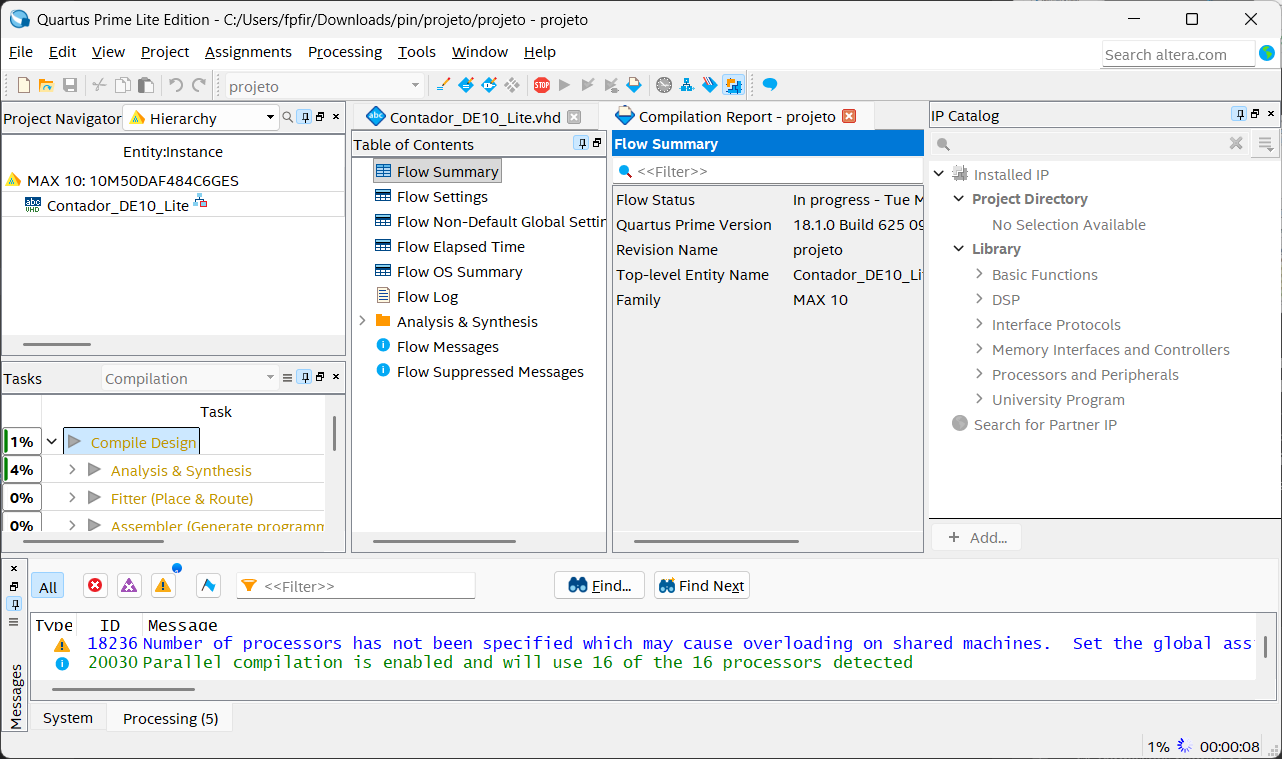
\includegraphics[width=0.95\textwidth]{image12.png}};
    \begin{scope}[x={(img.south east)},y={(img.north west)}]
        \node[calloutbox] (flow) at (0.68,0.08) {Relatório\\do fluxo};
        \draw[calloutarrow] (flow.north west) -- (0.50,0.74);
        \node[calloutbox] (tasks) at (0.25,0.25) {Etapas da\\compilação};
        \draw[calloutarrow] (tasks.north west) -- (0.08,0.42);
    \end{scope}
\end{tikzpicture}
\caption{Compilação em andamento no Quartus Prime.}
\label{fig:compilacao-andamento}
\end{figure}

\section{Gravação na placa}

Conecte a DE10-Lite ao computador pelo cabo USB e abra:

\begin{center}
\texttt{Tools > Programmer}
\end{center}

Na janela do Programmer, mostrada na Figura~\ref{fig:programmer-sem-hardware}, o arquivo \texttt{.sof} deve estar carregado e a opção \textit{Program/Configure} deve estar marcada. Se o campo de hardware aparecer como \textit{No Hardware}, clique em \textit{Hardware Setup}.

\caixaatencao{Se o campo de hardware continuar como \textit{No Hardware}, verifique o cabo USB, a alimentação da placa, o driver USB-Blaster e a seleção feita em \textit{Hardware Setup}. Sem o USB-Blaster selecionado, o botão \textit{Start} não grava o FPGA.}

\begin{figure}[H]
\centering
\calloutstyle
\begin{tikzpicture}
    \node[anchor=south west,inner sep=0] (img) at (0,0)
        {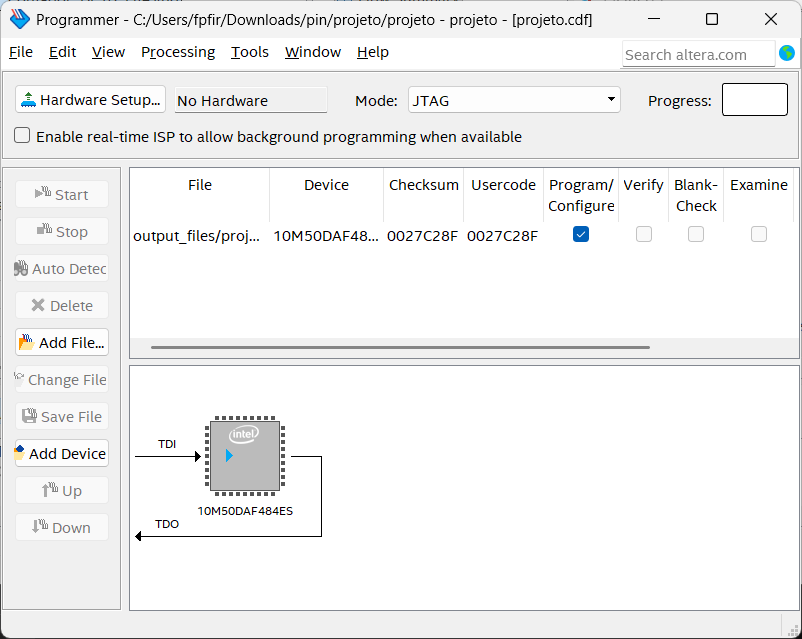
\includegraphics[width=0.78\textwidth]{image14.png}};
    \begin{scope}[x={(img.south east)},y={(img.north west)}]
        \node[calloutbox] (hw) at (0.36,0.77) {Selecionar\\hardware};
        \draw[calloutarrow] (hw.west) -- (0.19,0.84);
        \node[calloutbox] (sof) at (0.34,0.54) {Arquivo\\SOF};
        \draw[calloutarrow] (sof.west) -- (0.17,0.63);
        \node[calloutbox] (prog) at (0.84,0.36) {Programar};
        \draw[calloutarrow] (prog.north) -- (0.72,0.63);
    \end{scope}
\end{tikzpicture}
\caption{Programmer aberto antes da seleção do hardware USB-Blaster.}
\label{fig:programmer-sem-hardware}
\end{figure}

Na tela de configuração de hardware, a Figura~\ref{fig:hardware-setup-vazio} mostra a situação em que nenhum gravador está selecionado. Após conectar a placa e selecionar o gravador, o campo deve indicar \texttt{USB-Blaster [USB-0]}, como na Figura~\ref{fig:hardware-setup-usb}.

\imagemquartus{0.70}{image15.png}{Janela de configuração sem hardware selecionado.}{fig:hardware-setup-vazio}
\imagemquartus{0.70}{image16.png}{Janela de configuração com USB-Blaster selecionado.}{fig:hardware-setup-usb}

Depois que o USB-Blaster estiver selecionado, retorne ao Programmer. A Figura~\ref{fig:programmer-pronto} mostra a tela pronta para gravação; clique em \textit{Start}. Ao final, o progresso deve chegar a \textit{100\% (Successful)}, como mostrado na Figura~\ref{fig:programmer-sucesso}.

\begin{figure}[H]
\centering
\calloutstyle
\begin{tikzpicture}
    \node[anchor=south west,inner sep=0] (img) at (0,0)
        {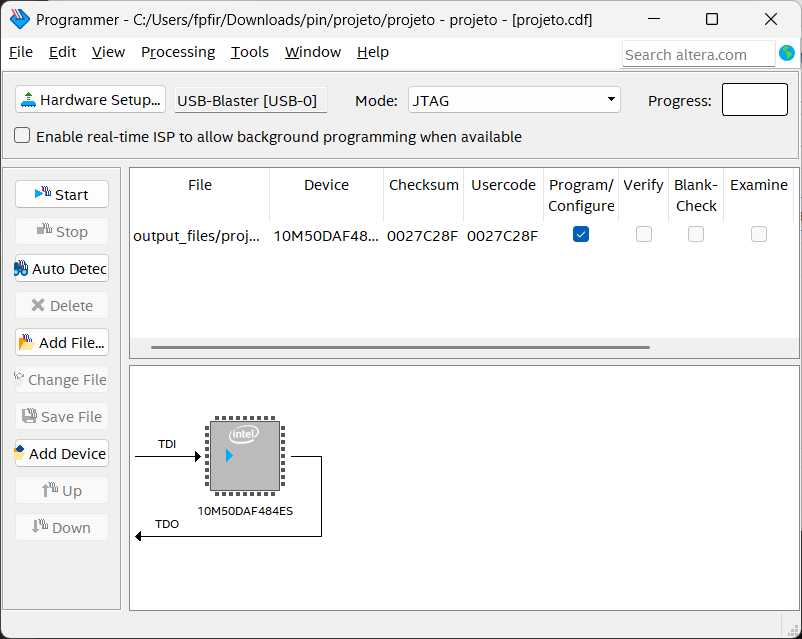
\includegraphics[width=0.78\textwidth]{image17.png}};
    \begin{scope}[x={(img.south east)},y={(img.north west)}]
        \node[calloutbox] (usb) at (0.55,0.34) {USB-Blaster\\selecionado};
        \draw[calloutarrow] (usb.north) -- (0.22,0.84);
        \node[calloutbox] (start) at (0.26,0.34) {Iniciar\\gravação};
        \draw[calloutarrow] (start.north west) -- (0.065,0.69);
    \end{scope}
\end{tikzpicture}
\caption{Programmer pronto para iniciar a gravação.}
\label{fig:programmer-pronto}
\end{figure}

\begin{figure}[H]
\centering
\calloutstyle
\begin{tikzpicture}
    \node[anchor=south west,inner sep=0] (img) at (0,0)
        {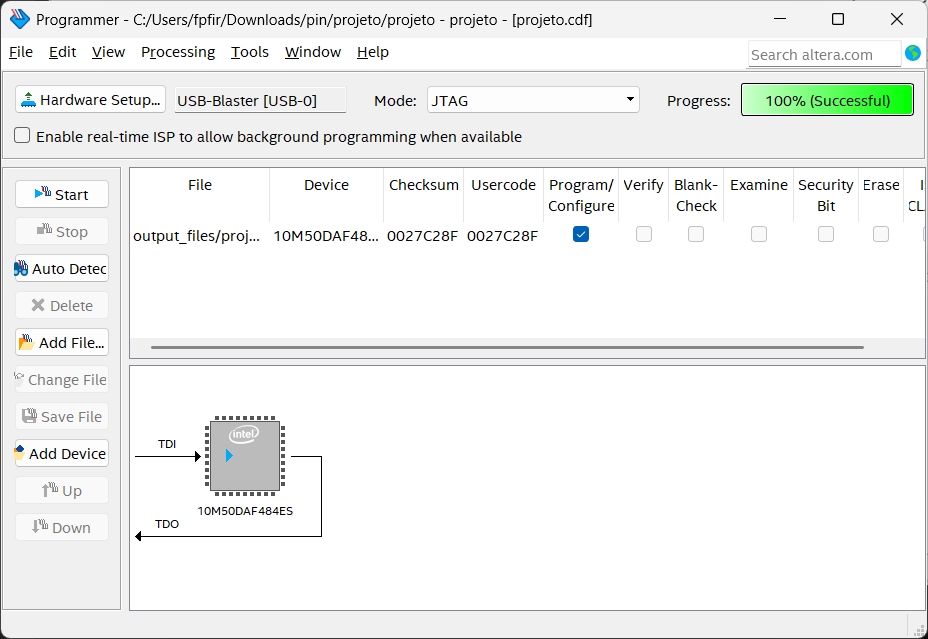
\includegraphics[width=0.86\textwidth]{image18.png}};
    \begin{scope}[x={(img.south east)},y={(img.north west)}]
        \node[calloutbox] (ok) at (0.62,0.28) {Gravação\\concluída};
        \draw[calloutarrow] (ok.east) -- (0.92,0.84);
    \end{scope}
\end{tikzpicture}
\caption{Gravação concluída com sucesso no kit DE10-Lite.}
\label{fig:programmer-sucesso}
\end{figure}

Para testar:

\begin{itemize}
    \item Pressione \texttt{KEY(0)} para zerar a contagem.
    \item Configure um valor BCD nas chaves \texttt{SW(7 downto 0)}.
    \item Pressione \texttt{KEY(1)} para carregar o valor.
    \item Observe a contagem nos displays \texttt{HEX1} e \texttt{HEX0}, como na Figura~\ref{fig:placa-teste}.
\end{itemize}

\begin{figure}[H]
\centering
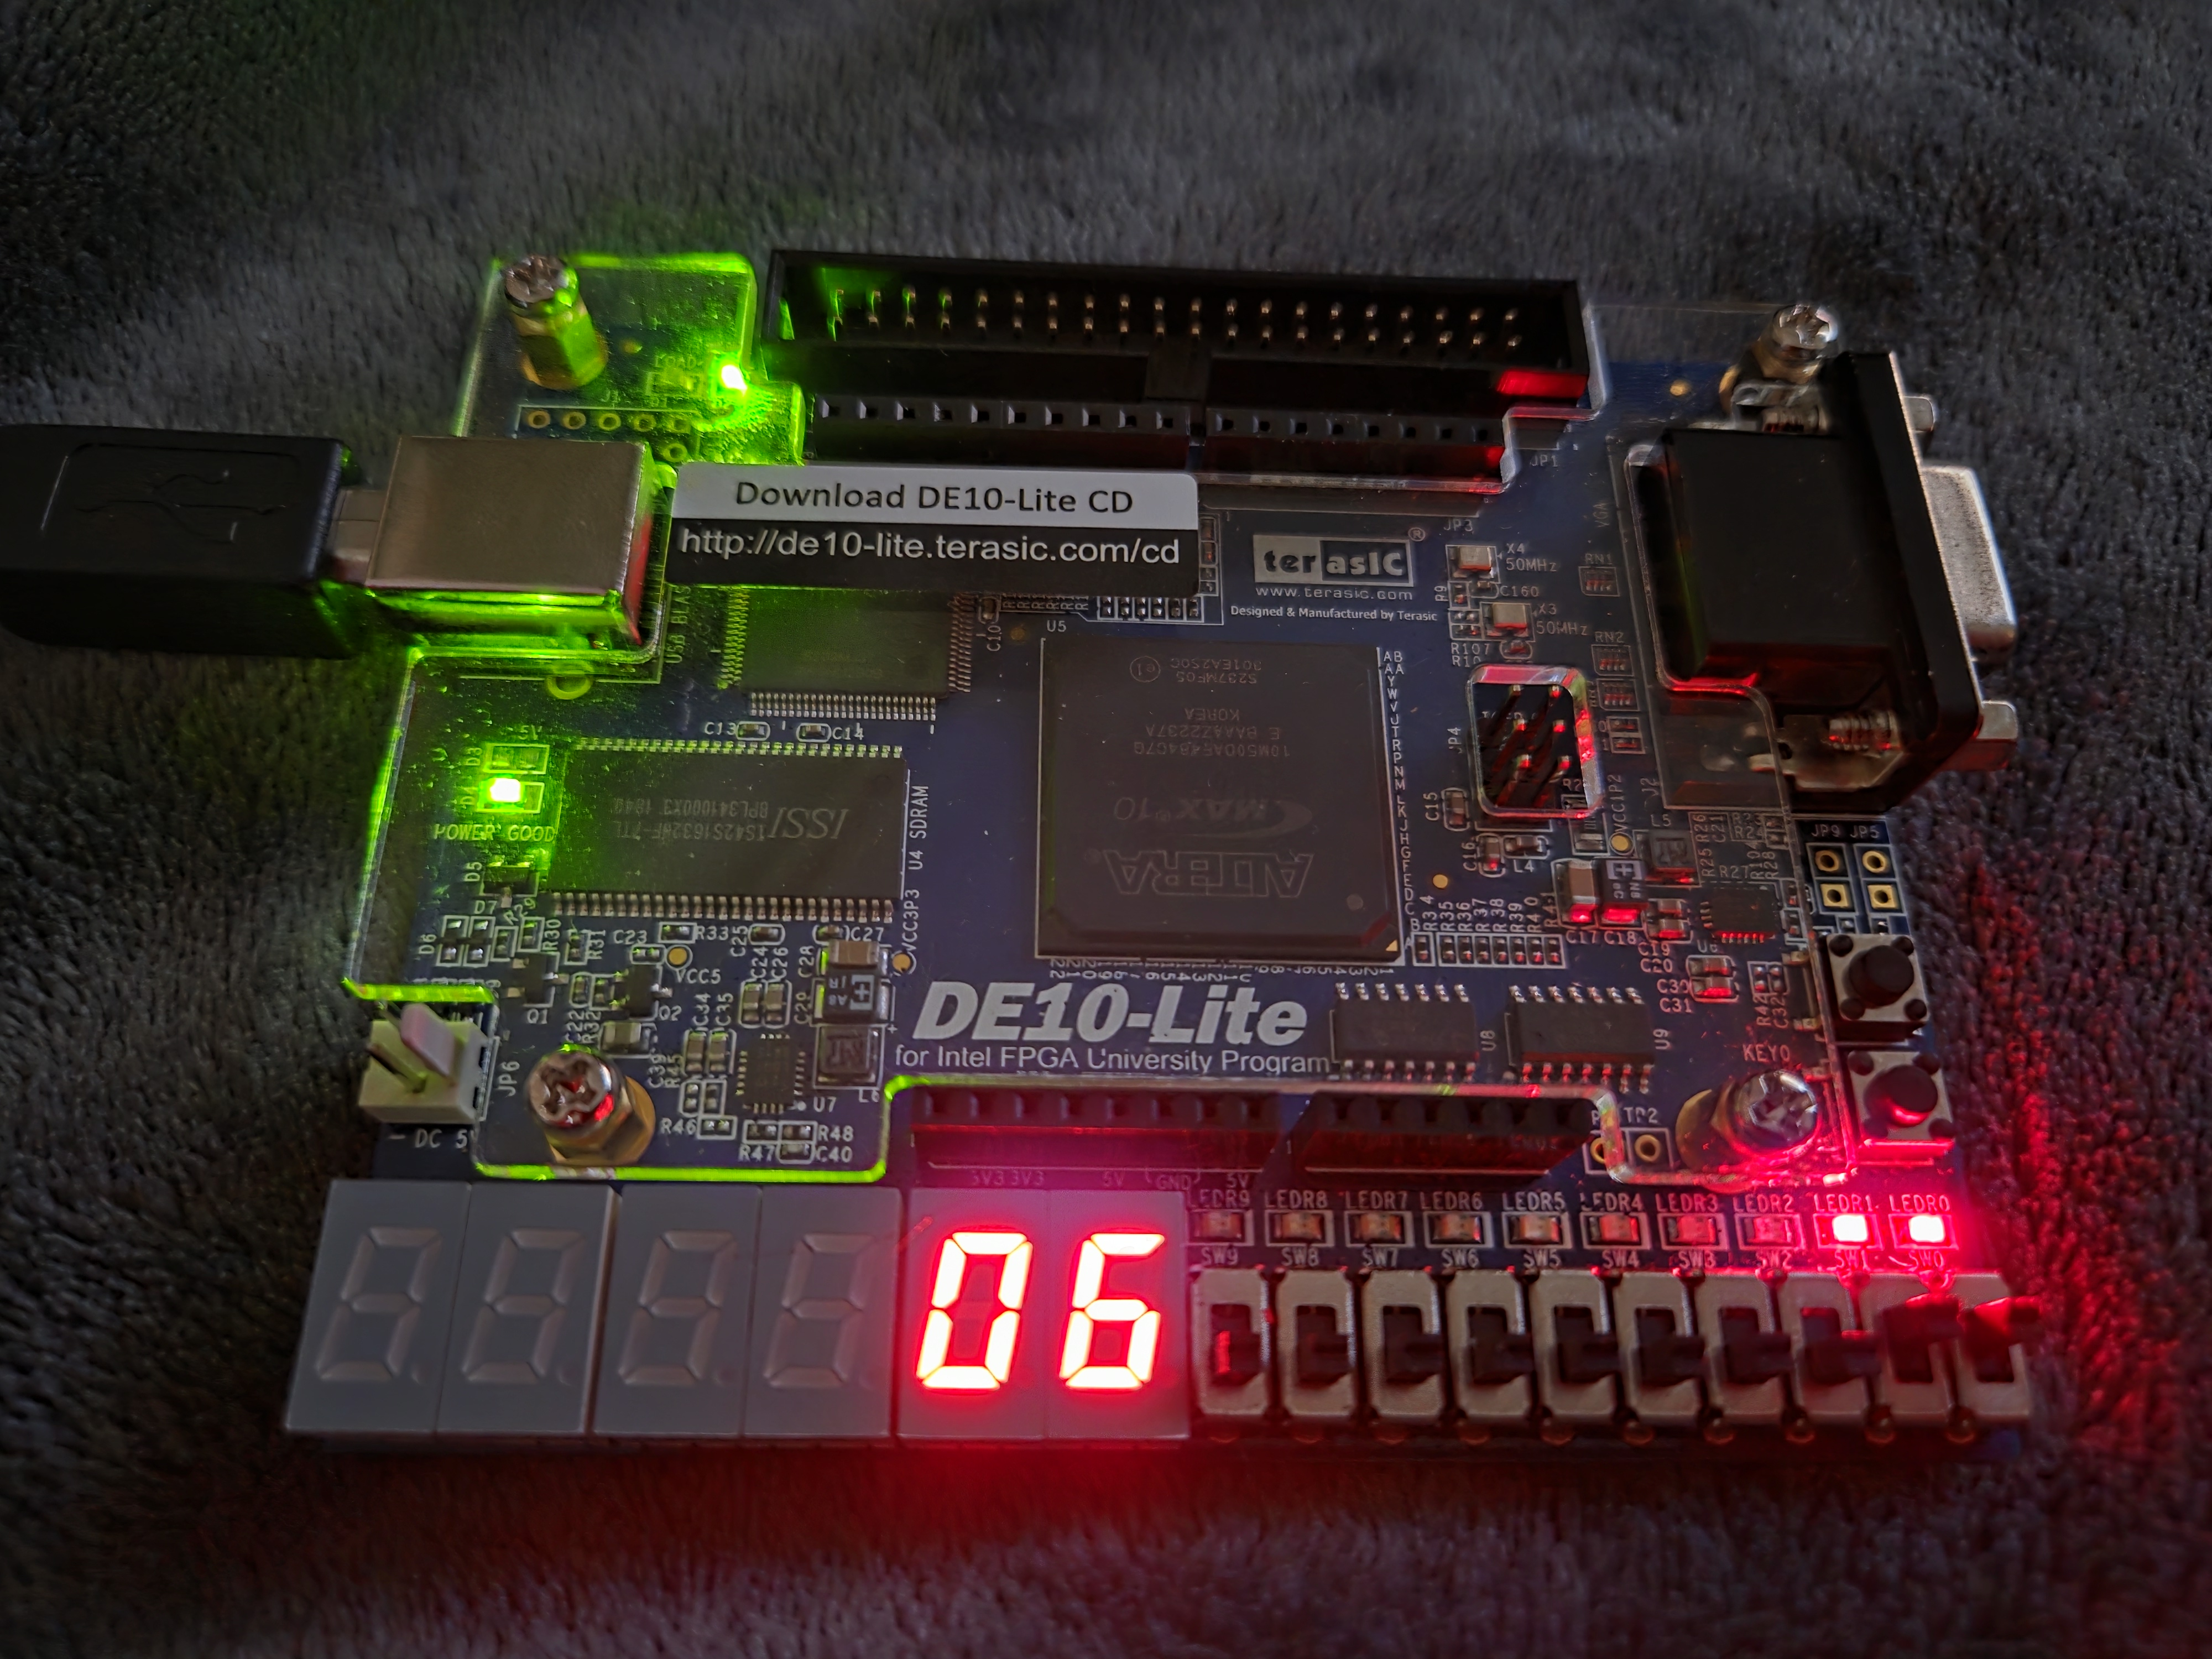
\includegraphics[angle=0,width=0.58\textwidth]{20260519_194343.jpg}
\caption{Kit DE10-Lite programado e exibindo a contagem nos displays de sete segmentos.}
\label{fig:placa-teste}
\end{figure}

\caixaresumo{Leitura rápida do teste}{
Com \texttt{KEY(0)} o valor volta para 00. Com \texttt{KEY(1)} o contador carrega o valor BCD definido em \texttt{SW(7 downto 0)}. Depois da carga, os displays \texttt{HEX1} e \texttt{HEX0} devem avançar a contagem decimal.
}

\section{Erros comuns}

A Tabela~\ref{tab:erros} resume problemas frequentes durante a criação, compilação e teste do projeto.

\begin{longtable}{p{0.33\textwidth}p{0.57\textwidth}}
\caption{Erros comuns durante a criação do projeto.}
\label{tab:erros}\\
\toprule
\rowcolor{tablehead}
\color{white}\textbf{Problema} & \color{white}\textbf{Possível solução} \\
\midrule
\endfirsthead
\caption[]{Erros comuns durante a criação do projeto (continuação).}\\
\toprule
\rowcolor{tablehead}
\color{white}\textbf{Problema} & \color{white}\textbf{Possível solução} \\
\midrule
\endhead
\rowcolors{2}{tablerow}{white}
O Quartus não encontra a entidade principal & Verifique se o nome da entidade VHDL é igual ao campo \textit{Top-level entity}. \\
Erro de pino não atribuído & Abra o Pin Planner ou confira se o sinal possui \texttt{set\_location\_assignment} no arquivo \texttt{.qsf}. \\
Erro de padrão elétrico & Confira se cada sinal possui \texttt{IO\_STANDARD}. Para chaves, clock, LEDs e displays, use \texttt{3.3-V LVTTL}; para botões, use \texttt{3.3 V SCHMITT TRIGGER}. \\
Display de sete segmentos parece invertido & Lembre-se de que os segmentos são ativos em nível baixo: \texttt{0} acende e \texttt{1} apaga. \\
Carga paralela não mostra o valor esperado & Confira se as chaves estão em BCD válido: unidades em \texttt{SW(3 downto 0)} e dezenas em \texttt{SW(7 downto 4)}, cada grupo de 0 a 9. \\
\bottomrule
\end{longtable}

\section{Atividade proposta}

Modifique o contador para:

\begin{itemize}
    \item usar \texttt{SW(9)} como habilitação da contagem;
    \item manter o valor congelado quando \texttt{SW(9) = '0'};
    \item piscar \texttt{LEDR(9)} a cada pulso de um segundo.
\end{itemize}

\caixaresumo{Desafio extra}{
Depois de concluir a atividade, altere o projeto para contar de 00 a 59, como em um cronômetro simples. Essa mudança exige limitar as unidades a 9 e as dezenas a 5.
}

\section{Conclusão}

Neste roteiro, foi criado um projeto no Quartus Prime Lite para a placa DE10-Lite, selecionando o dispositivo correto, definindo um top-level design próprio em VHDL e associando os sinais lógicos aos pinos físicos do FPGA. O arquivo \texttt{DE10\_LITE\_Golden\_Top.v}, quando gerado, foi usado apenas como referência para os nomes das portas da placa. Esse procedimento é a base para projetos digitais maiores, pois todo circuito implementado na DE10-Lite depende da correta relação entre o código HDL e os recursos físicos do kit.

\end{document}
